\subsubsection{Packet Loss and its effect on download speeds}

% Better graph needed
\begin{center}
	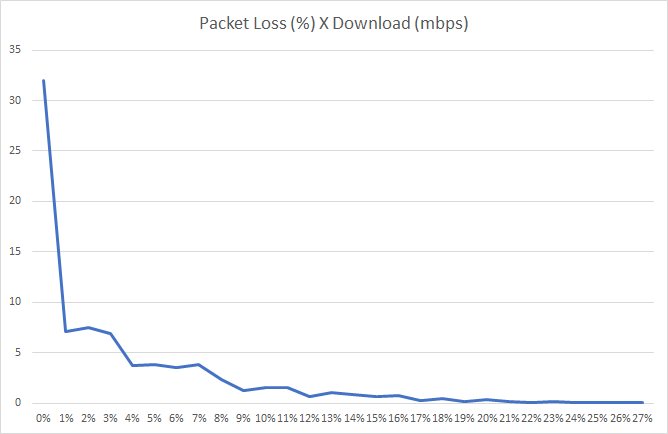
\includegraphics[scale=0.6]{PL_Download}
	\begin{figure}[h]
	 	\caption{Graph displaying effect of packet loss on download speeds}
	\end{figure}		
\end{center}






The graph above shows the download speed measured in Mbps against the increasing rate of packet loss, as you can see the download rate only reaches around 25\%, this is due to the connection test failing at anything above. The tests were performed by using Iperf on the localhost as to reduce any degradation that may exists already in an existing network.

My initial hypothesis for the sharp decreases in packet loss from 0\% to 1\% is due to the congestion control mechanisms built into TCP. TCP as mentioned in the background section allows for multiple devices to co-exist on a network and needs to dynamically balance network resources for every client, it performs this through congestion control algorithms where packet loss in this aspect is assumed as a sign of congestion to the algorithm where it adapts by reducing its transfer rate each time a packet is lost, this means the transfer rate drastically reduces until it reaches a platform. The transfer rate is dictated by a few factors, one known as the congestion window (Cwnd) and the advertised size of the receiving window (Rwnd). The overall window size is the smaller of these two numbers, and the smaller the window size, the less packets can be send in one time frame. The congestion window therefore is reduces every time packet loss is detected. 

The test devised to prove this hypothesis will involve once again an iperf client/server where a packet is dropped after a time period while the congestion window size is tracked. Below is a graph showing the result of a test spanning 10 seconds where a single incoming packet was dropped every 1 second, the graph is measuring Cwnd sizes on the y axis and Time on the x axis.

%Graph
\begin{center}
	\begin{tikzpicture}[]
		\begin{axis}[
			width=\linewidth,
			height=10cm, 
			grid=major,
			xlabel=Time,
			ylabel=Cwnd]
			\addplot table [mark=*, search path=csv_data, col sep=comma]{PacketLossCwnd.csv};
			
		 \end{axis}
 	\end{tikzpicture}
\end{center}

As you can see around the 1 second mark there are almost identical drops in the Cwnd size, this demonstrates that packet loss causes the congestion window to reduce in size and if packet loss is substantial enough can cause a huge drop in transfer rates.

Please also note the initial increase in transfer rate, this is displayed in the graph below:

\begin{center}
	\includegraphics[scale=0.6]{TCP_Slow_Start}
	\begin{figure}[h]
	 	\caption{Close up of the initial start}
	\end{figure}		
\end{center}

This is known as the TCP Slow start and this is used by the protocol to naturally align itself into the network eco-system, it starts off with a modest transfer rate to prevent situations where an initial abnormally large transfer rate would fill buffers and cause network congestion and adjusts by incorporating the techniques explained above to manually adjust its transfer rate to fit naturally into the current network.
 